\section{Dokumentengeschichte}
\begin{table}[h]
 \begin{tabular}{|l|l|p{4cm}|}
 \hline
 Zeitraum & PL/Autor(en) & Änderungen \\
 \hline
 Wintersemester 2017 & Feurich, Dustin &
Kapitel erstellt und Software dokumentiert \newline
  \\
 \hline
 \end{tabular}
 \caption{Dokumentengeschichte}
 \end{table}

\section{Aufgabe der Komponente}



\section{Architektur}

\subsection{Überlick}\label{ch:offlineoverview}

In der folgenden Grafik sind alle Bestandteile der Bluetooth Komponente von SharkNet abgebildet.
\begin{figure}[H]
	\centering
	\hspace*{1cm}
	\makebox[\linewidth][c]{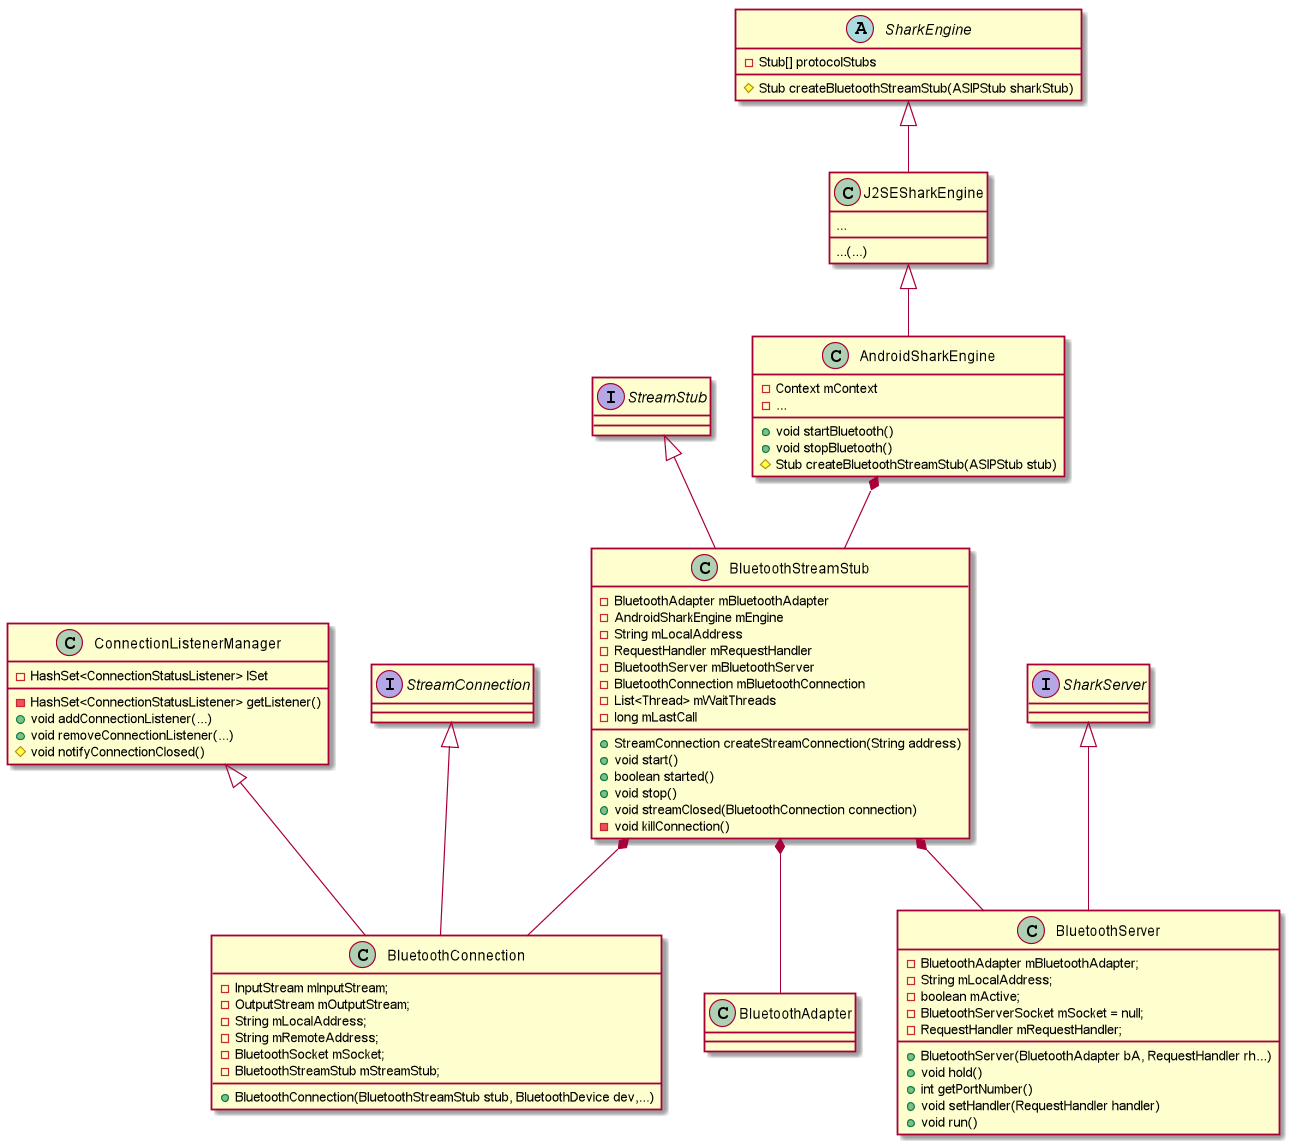
\includegraphics[width=1.1\linewidth]{bluetooth/images/bluetoothGesamt.png}}%
	\caption{Die Bluetooth Klassen im Überblick}
	\label{fig:bluetoothAll}
\end{figure}

\newpage

In der folgenden Grafik sind alle Bestandteile der WifiDirect Komponente von SharkNet abgebildet.
\begin{figure}[H]
	\centering
	\hspace*{1cm}
	\makebox[\linewidth][c]{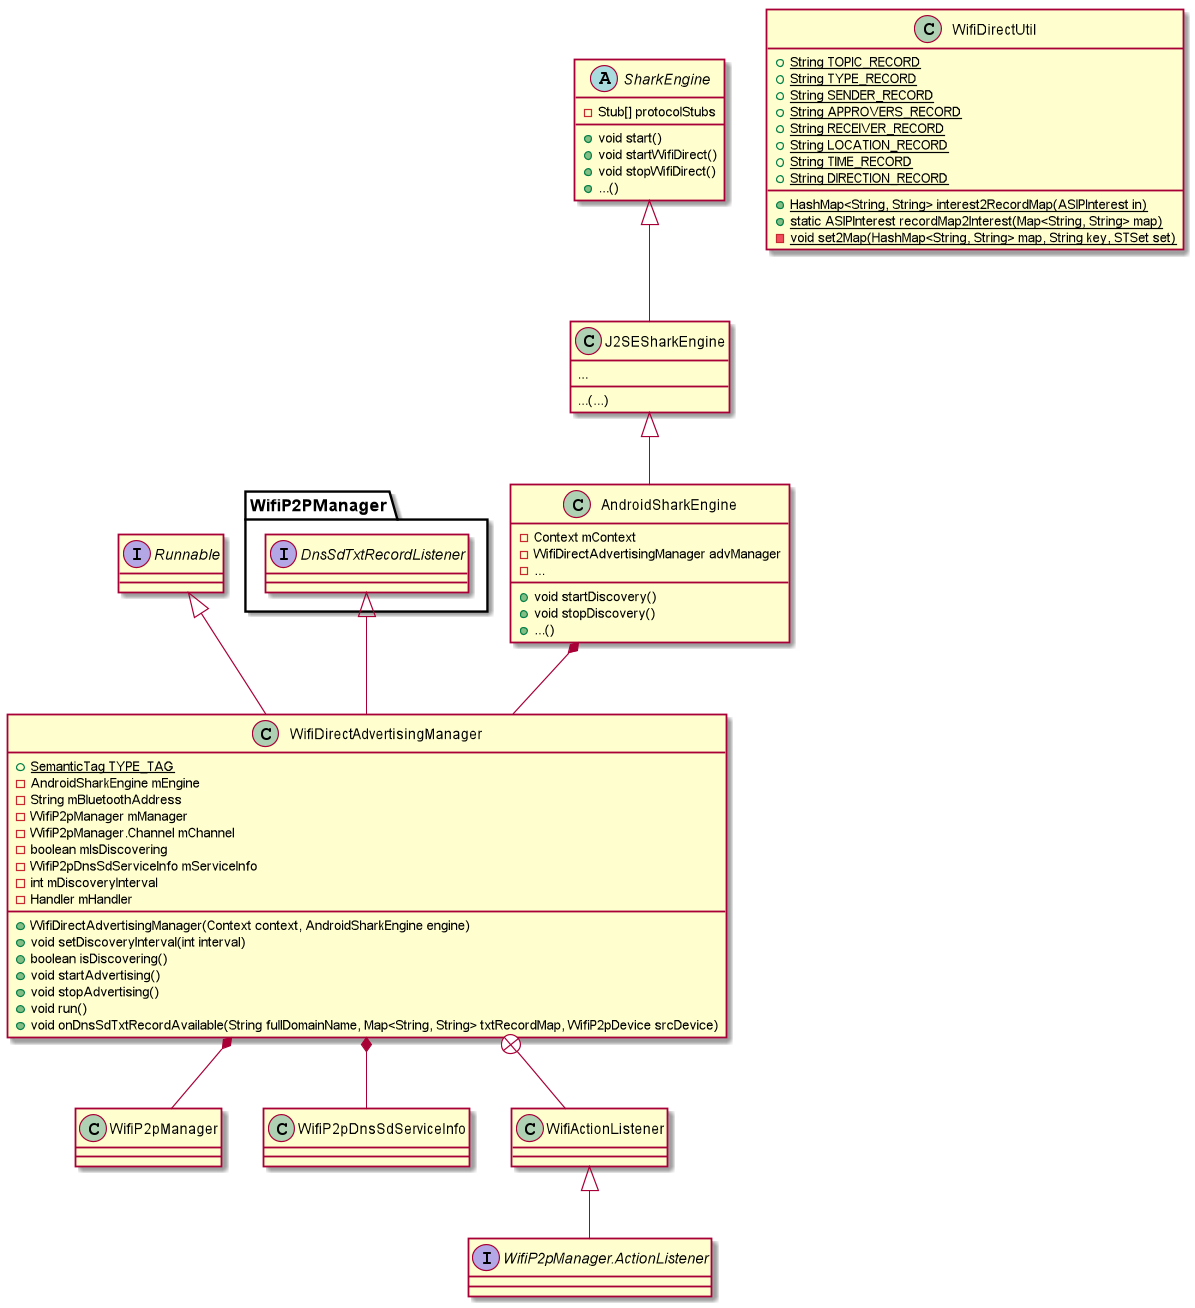
\includegraphics[width=1.1\linewidth]{wifi/images/wifiDirectGesamt.png}}%
	\caption{Die WifiDirect Klassen im Überblick}
	\label{fig:wifiAll}
\end{figure}

\newpage

In der folgenden Grafik sind alle Bestandteile der Radar Komponente abgebildet.
\begin{figure}[H]
	\centering
	\hspace*{1cm}
	\makebox[\linewidth][c]{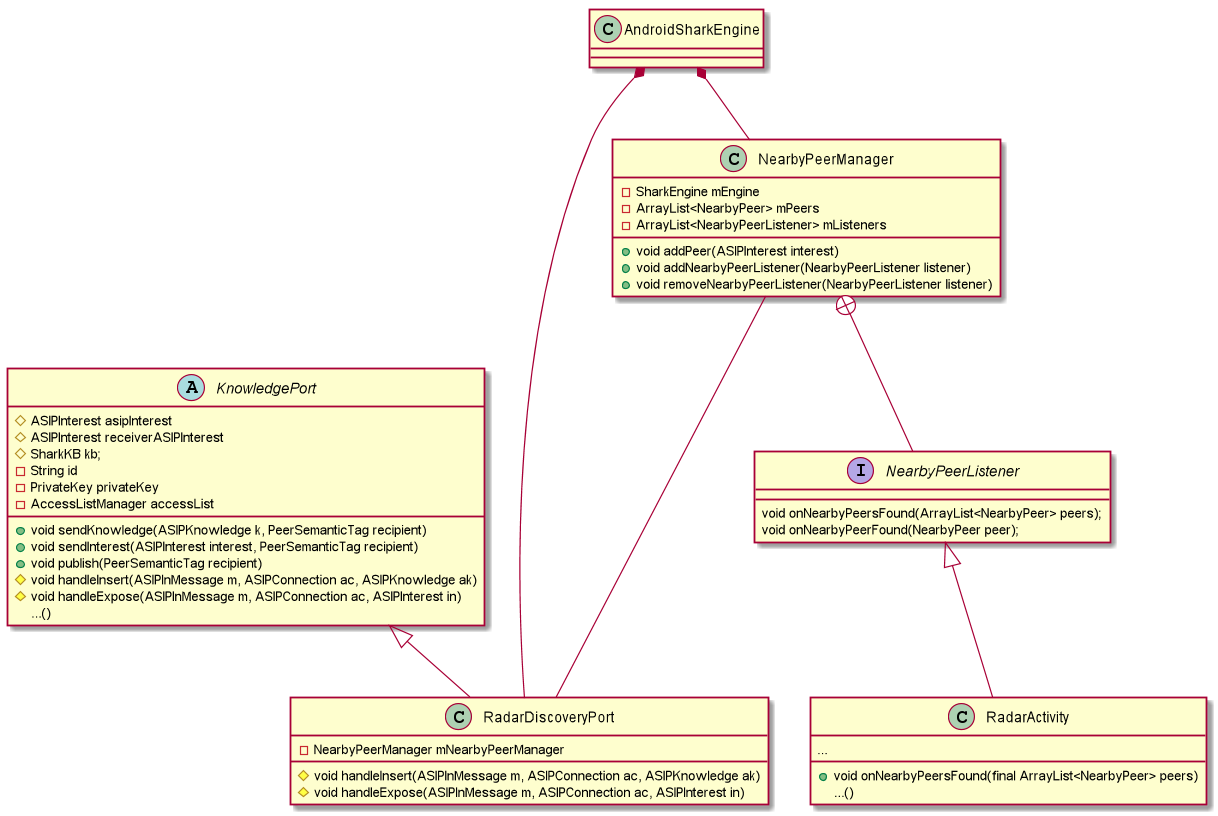
\includegraphics[width=1.1\linewidth]{bluetooth/images/radar.png}}%
	\caption{Die Radar Klassen im Überblick}
	\label{fig:radarAll}
\end{figure}

\newpage

Im folgenden Aktivitätsdiagramm wird das Versenden von Nachrichten per Broadcast abgebildet
\begin{figure}[H]
	\centering
	\hspace*{1cm}
	\makebox[\linewidth][c]{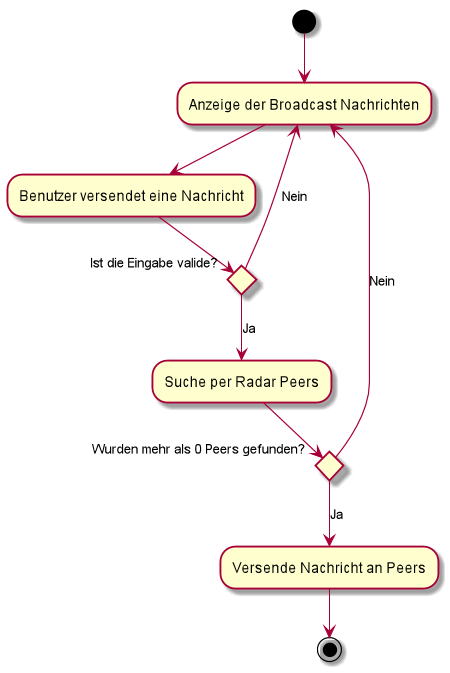
\includegraphics[width=0.5\linewidth]{broadcast/images/broadcastSend.png}}%
	\caption{Versenden von Nachrichten per Broadcast in SharkNet}
	\label{fig:broadcastSend}
\end{figure}

\newpage

Im folgenden Aktivitätsdiagramm wird das Empfangen von Nachrichten per Broadcast abgebildet
\begin{figure}[H]
	\centering
	\hspace*{1cm}
	\makebox[\linewidth][c]{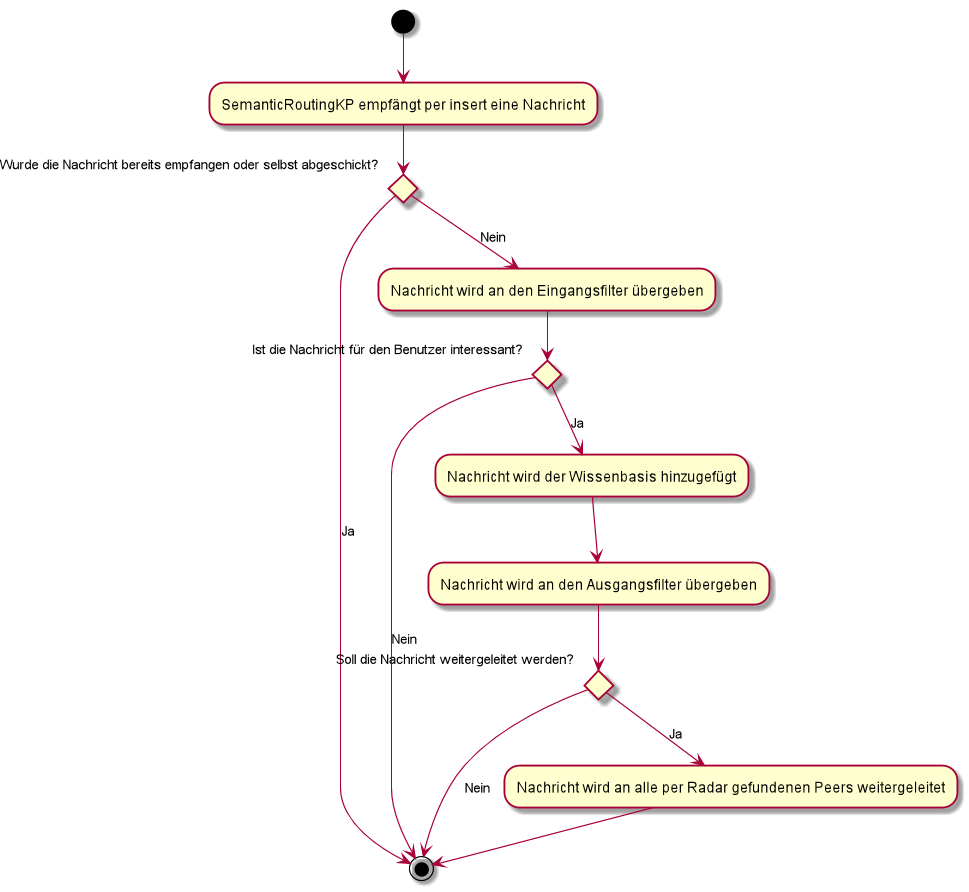
\includegraphics[width=0.9\linewidth]{broadcast/images/broadcastReceive.png}}%
	\caption{Empfangen von Nachrichten per Broadcast in SharkNet}
	\label{fig:broadcastReceive}
\end{figure}

\newpage


\subsection{Schnittstellendefinitionen}\label{ch:offlineinterfaces}


\section{Nutzung}
\subsection{Code}
Der aktuelle Code kann unter\\ \url{https://github.com/OpenHistoricalDataMap/OfflineMaps}\\ bezogen werden. Die Struktur des Codes wurde bereits in Kapitel \ref{ch:offlineoverview} erläutert und grafisch dargestellt.

\subsection{Deployment / Runtime}



\section{Qualitätssicherung}



\subsection{Test}


\section{Vorschläge / Ausblick}
